\chapter{Convertitore Tensione-Frequenza}

%--------------------------------------------------------------------------------------------

Si vuole ora progettare il circuito per la generazione del segnale $f_{clk}$, con le
specifiche ottenute dal capitolo precedente, ovvero:

\begin{itemize}
    \item Frequenza minima: $\approx 14\ kHz$;
    \item Frequenza massima: $\approx 3.6\ MHz$;
    \item Livello logico basso: $0\ V$;
    \item Livello logico alto: $+5\ V$;
\end{itemize}

%--------------------------------------------------------------------------------------------

\subsection*{Principio di Funzionamento}

%--------------------------------------------------------------------------------------------

Ciò di cui abbiamo bisogno è un circuito in grado di convertire una tensione in un segnale
a onda rettangolare con frequenza proporzionale alla tensione stessa, ovvero un convertitore
tensione-frequenza.

In commercio è possibile trovare diversi chip in grado di svolgere questa funzione
semplicemente aggiungendo una manciata di componenti di contorno, anche se la maggior
parte di questi non arriva a coprire l'intero range di funzionamento di cui abbiamo bisogno
(come ad esempio il noto LM331 \cite{lm331}). Nel nostro caso si utilizza un VFC110
\cite{vfc110}, circuito integrato che vanta un'ottima linearità e capace di fornire una
frequenza di $4\ MHz$ in uscita con una corrispondente tensione in ingresso di $10\ V$,
esattamente ciò che la nostra applicazione richiede.

\begin{figure}[H]
    \centering
    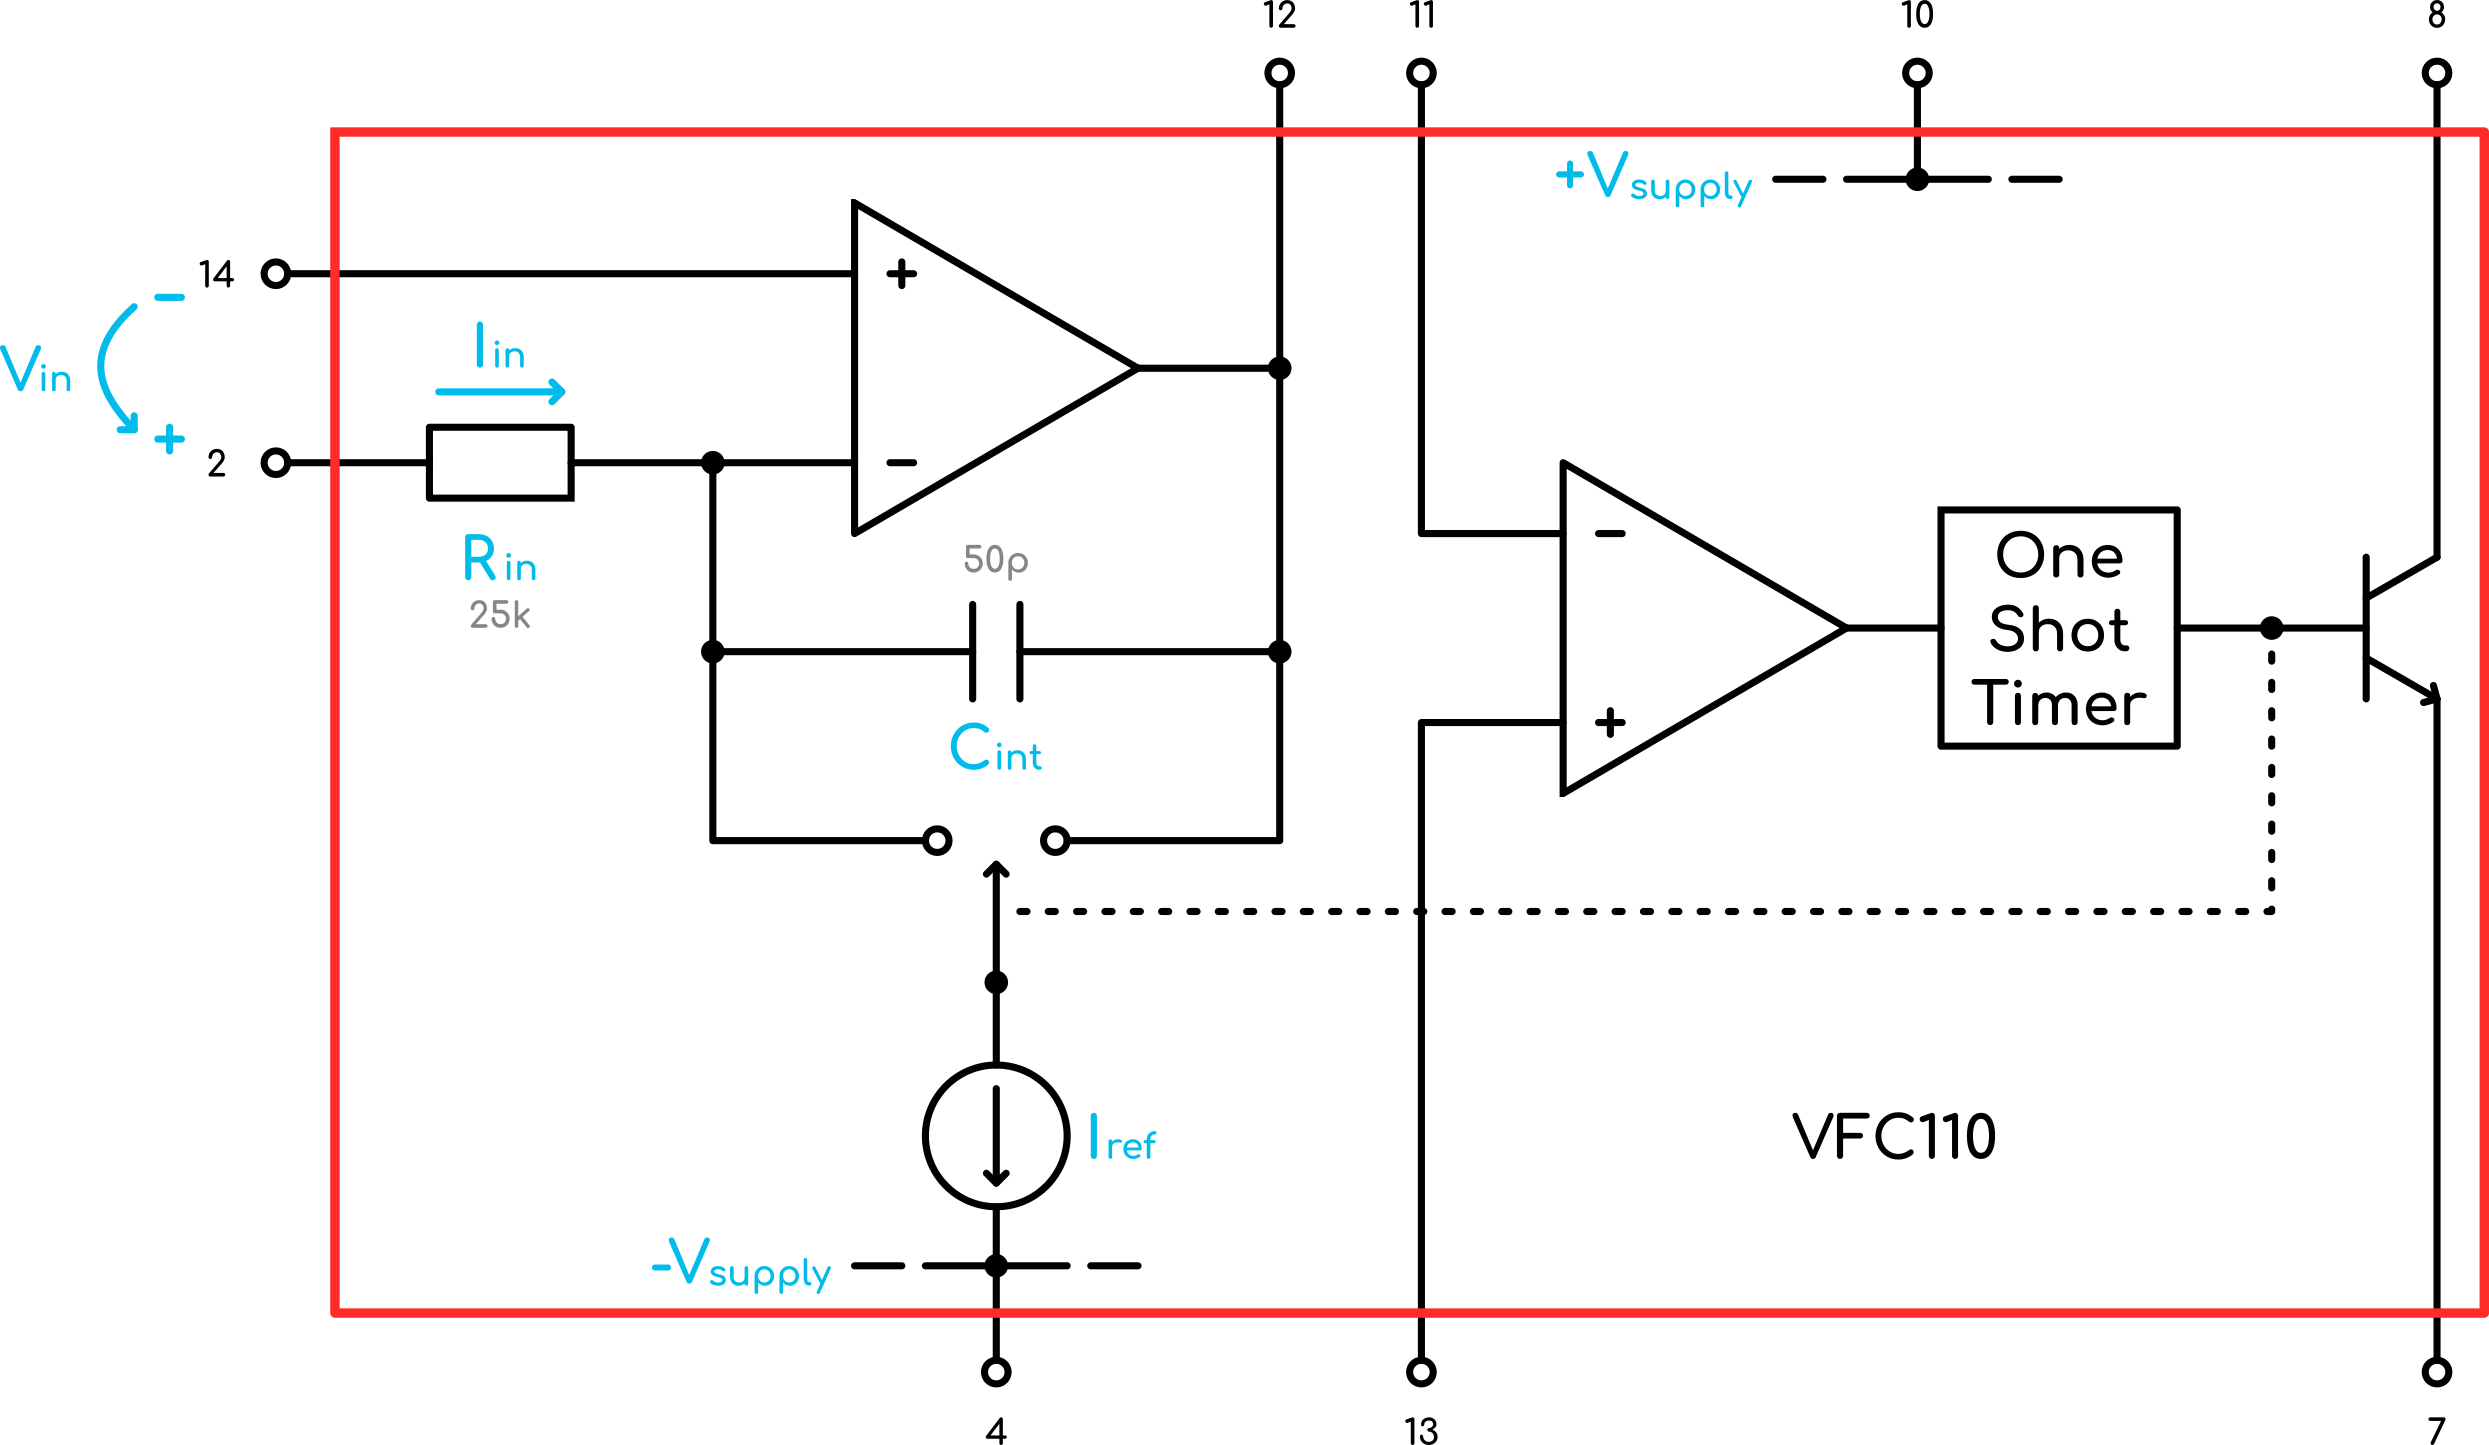
\includegraphics{circuits/vfc110_internal.png}
    \caption{Estratto utile della struttura interna di un VFC110}
    \label{vfc110_internal}
\end{figure}

Il cuore del circuito (figura \ref{vfc110_internal}) consiste in un operazionale configurato
come integratore, con tensione di uscita proporzionale alla carica immagazzinata nella sua
capacità di feedback $C_{int}$. Una tensione in ingresso $V_{in}$ sviluppa una corrente
$I_{in}=\frac{V_{in}}{R_{in}}$ che viene forzata in $C_{int}$, causando quindi una rampa
decrescente in uscita. Arrivati a $0\ V$ il comparatore scatta, attivando il timer one-shot.
Quindi un generatore di corrente $I_{ref}$ (dal valore di circa $1\ mA$) viene connesso
all'ingresso dell'integratore per un periodo di durata pari a $T_{OS}$, causando una rampa
crescente in uscita. Infine il ciclo ricomincia.

\begin{figure}[H]
    \centering
    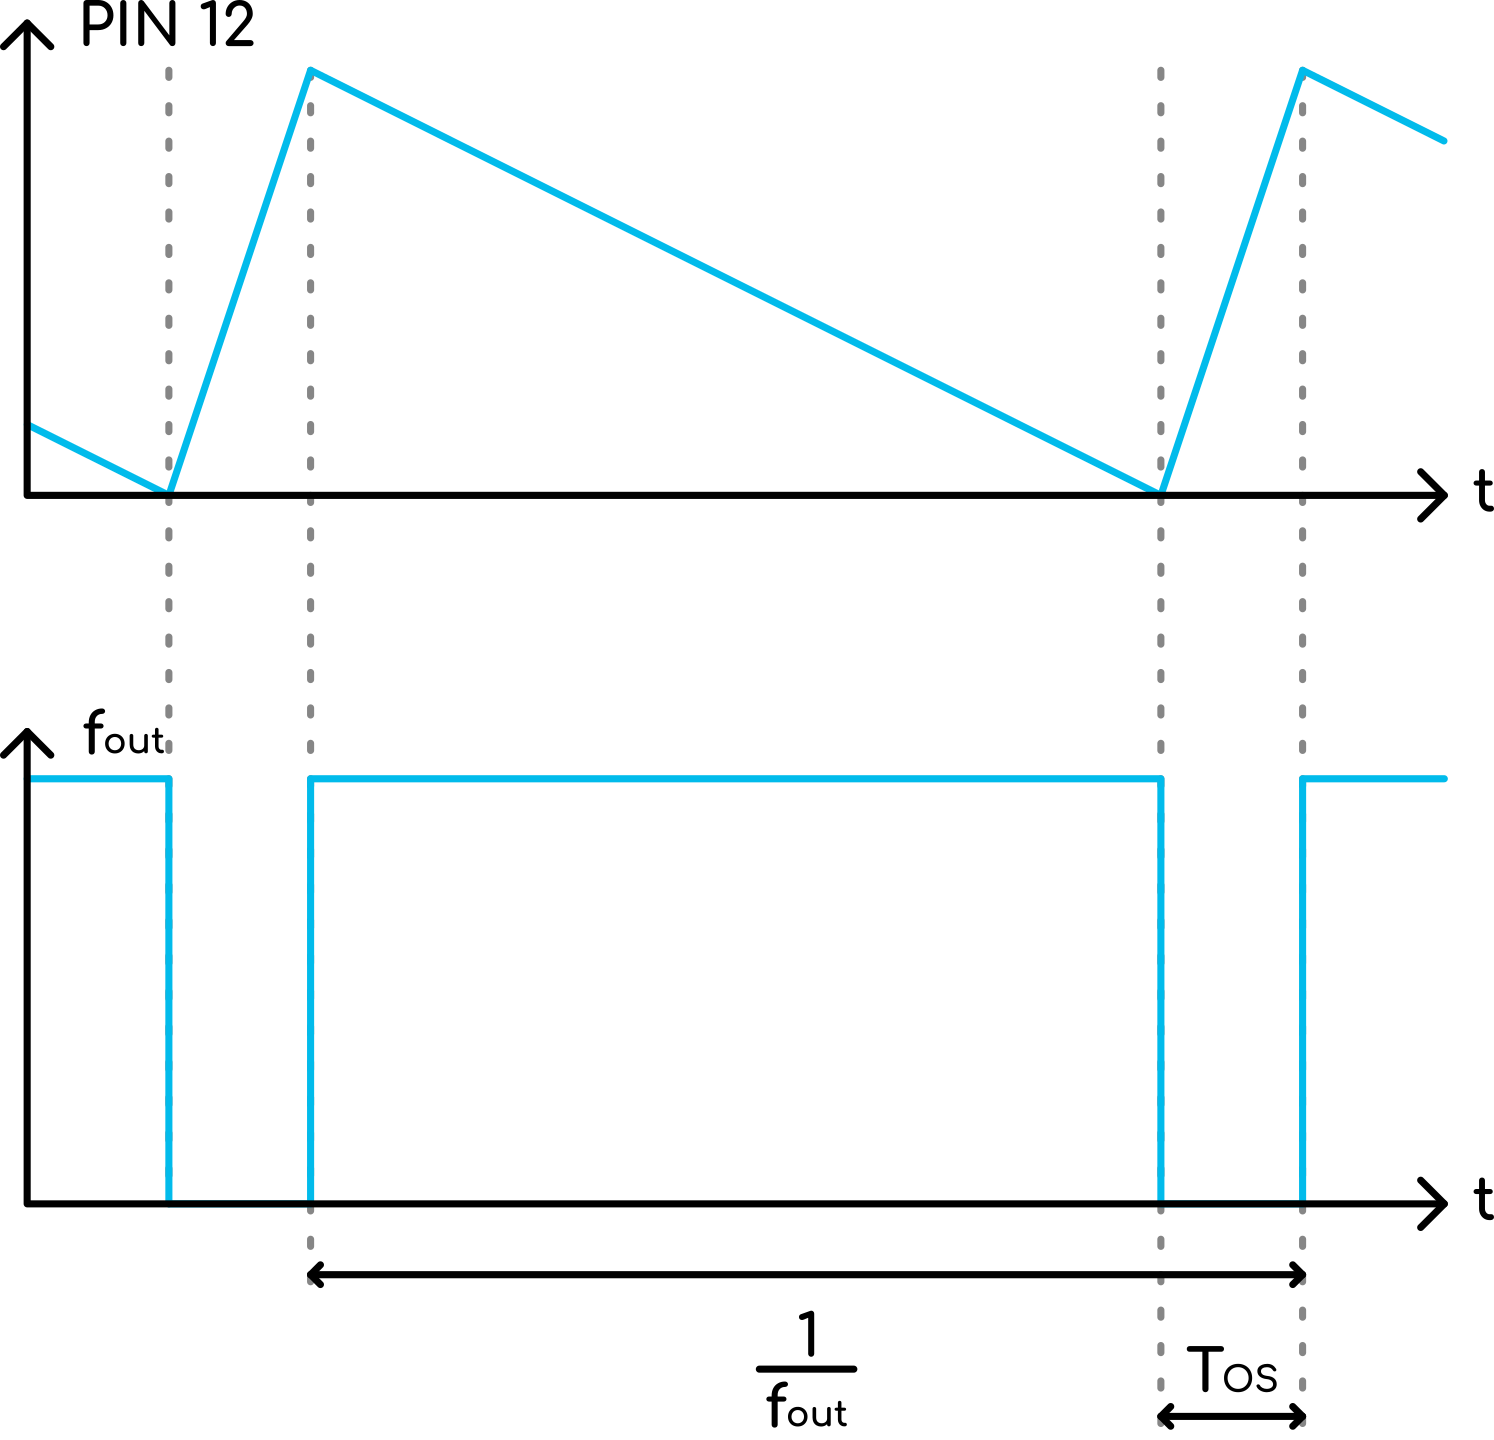
\includegraphics{graphs/integrator_behaviour.png}
    \caption{Forme d'onda teoriche del VFC110}
    \label{integrator_behaviour}
\end{figure}

Per uno studio più approfondito sul funzionamento del VFC110 si consiglia la lettura del
datasheet del componente, dal quale si ricava anche la configurazione del circuito utilizzato
per sfruttare l'intero range offerto (figura \ref{VFC_circuit}). Si modificano solo i valori
di alimentazione, sostituendoli con quelli dello standard scelto ($\pm 12\ V$).

\begin{figure}[H]
    \centering
    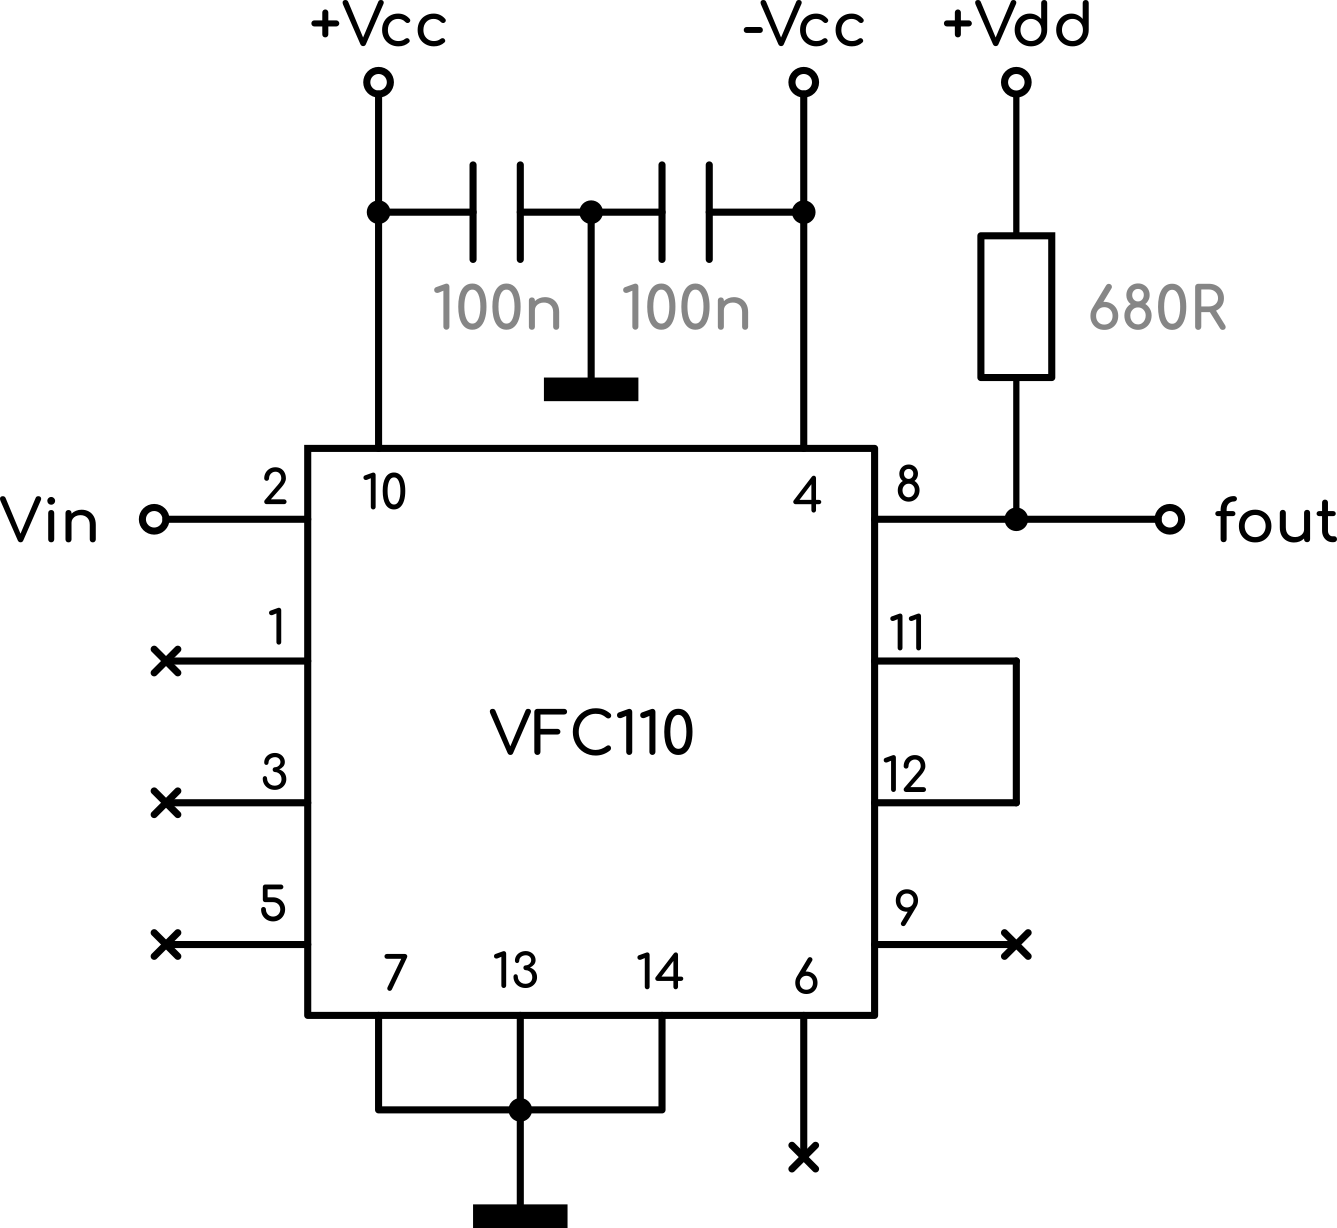
\includegraphics{circuits/VFC_circuit.png}
    \caption{Schema elettrico del VFC110 utilizzato}
    \label{VFC_circuit}
\end{figure}

Si noti che gli unici componenti aggiunti sono condensatori di filtro e un resistore di
pull-up per l'uscita a collettore aperto.

Si riportano le relazioni tra le grandezze in gioco:

\begin{displaymath}
    I_{in}=I_{ref}\cdot\delta\ [A]
    \qquad
    \rightarrow
    \qquad
    \delta=\frac{I_{in}}{I_{ref}}=\frac{V_{in}}{R_{in}\cdot I_{ref}}\ [\%]
\end{displaymath}

\begin{displaymath}
    \frac{V_{in}}{R_{in}}=I_{ref}\cdot f_{out}\cdot T_{OS}\ [A]
    \qquad
    \rightarrow
    \qquad
    f_{out}=\frac{V_{in}}{R_{in}\cdot I_{ref}\cdot T_{OS}}=\frac{\delta}{T_{OS}}\ [Hz]
\end{displaymath}

%--------------------------------------------------------------------------------------------

\subsection*{Risultati Pratici e Misure}

%--------------------------------------------------------------------------------------------

Si procede quindi alla verifica del corretto funzionamento del circuito. Il setup di
misura utilizzato viene riportato in figura \ref{mis_VFC}.

\begin{figure}[H]
    \centering
    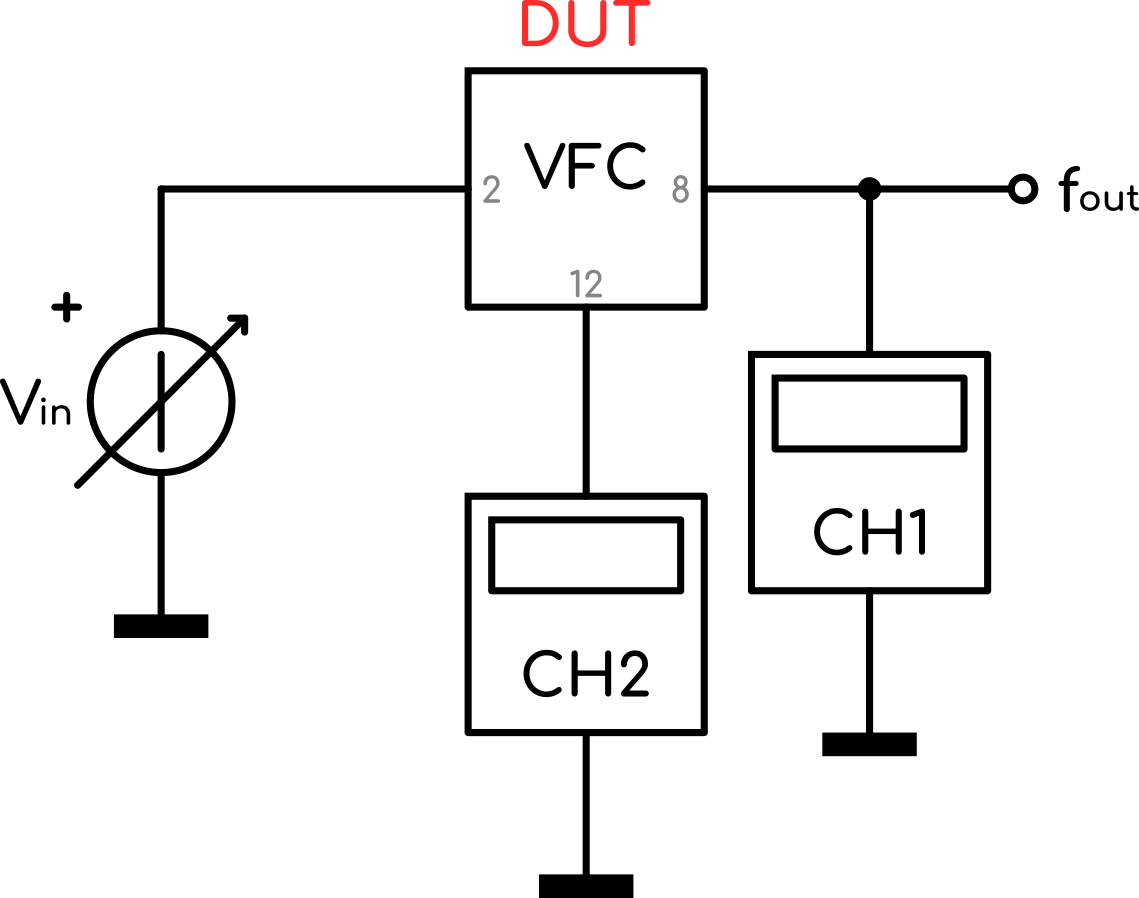
\includegraphics{block_diagrams/mis_VFC.png}
    \caption{Circuito di misura del VFC}
    \label{mis_VFC}
\end{figure}

Possiamo innanzitutto verificare che il comportamento dell'integratore corrisponde a quello
descritto nel paragrafo precedente, e si nota che la durata del periodo basso di $f_{out}$
si estende lungo il tratto di rampa crescente, come in figura \ref{integrator_behaviour}.

\begin{figure}[H]
    \centering

    \begin{subfigure}{.5\textwidth}
        \centering
        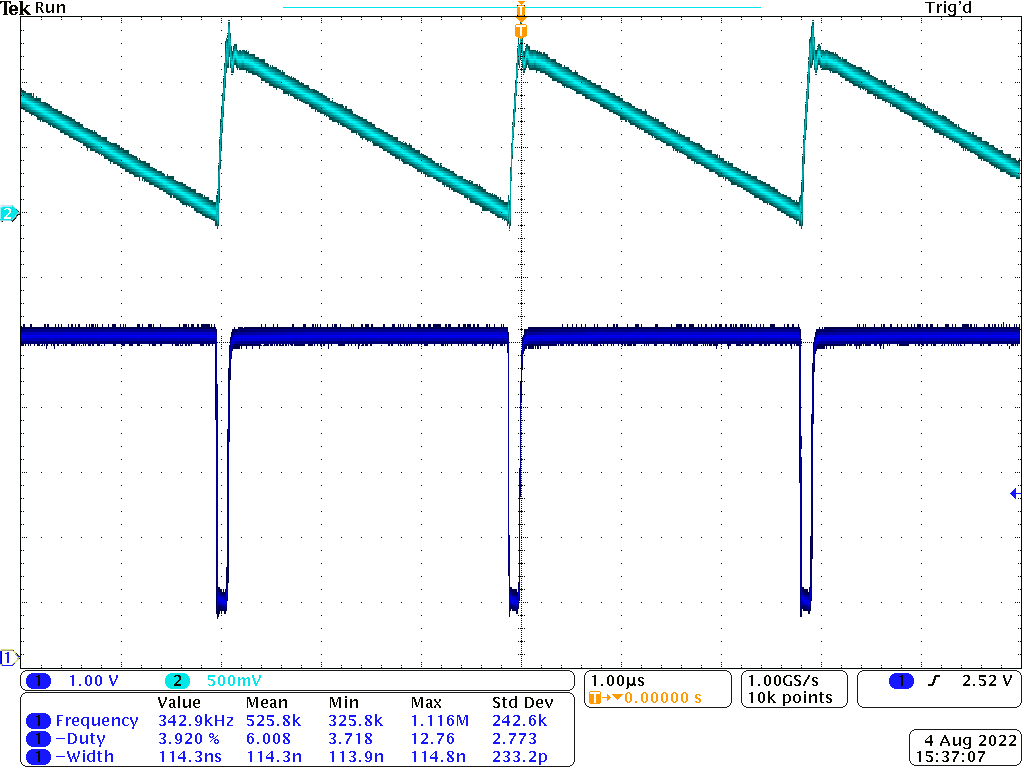
\includegraphics[scale = 0.2]{acquisitions/VFC_1V.png}
        \caption{$V_{in}=1\ V$}
        \label{acq_vfc110_1v}
    \end{subfigure}%
    \begin{subfigure}{.5\textwidth}
        \centering
        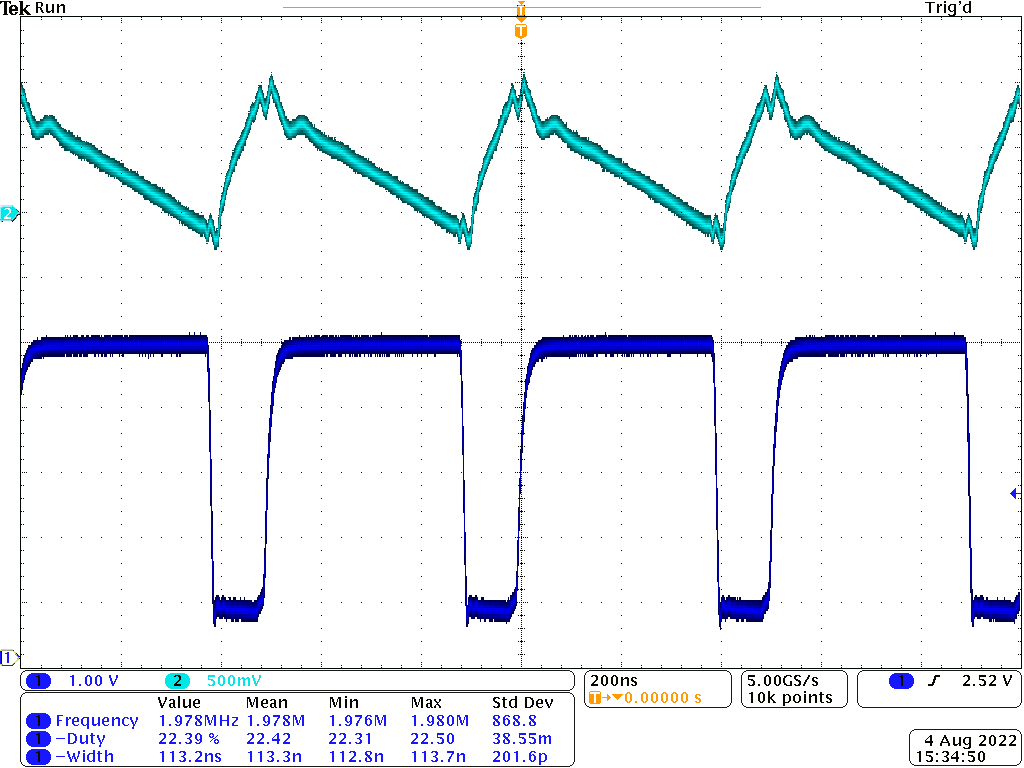
\includegraphics[scale = 0.2]{acquisitions/VFC_5V.png}
        \caption{$V_{in}=5\ V$}
        \label{acq_vfc110_5v}
    \end{subfigure}
    \begin{subfigure}{.5\textwidth}
        \centering
        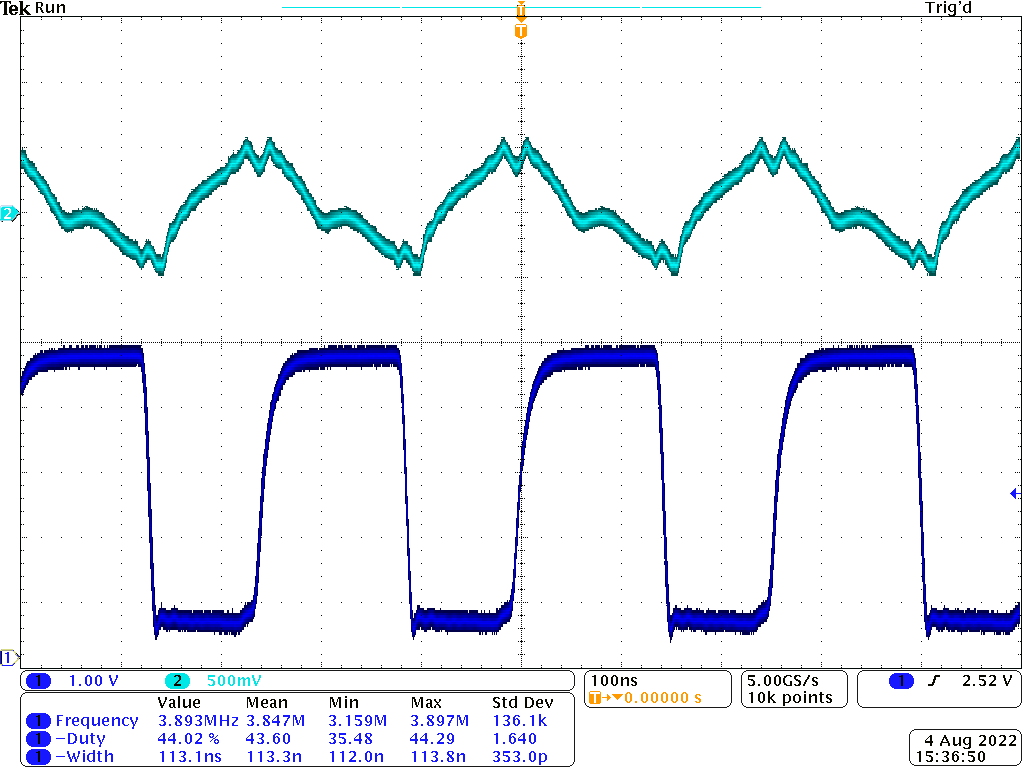
\includegraphics[scale = 0.2]{acquisitions/VFC_10V.png}
        \caption{$V_{in}=10\ V$}
        \label{acq_vfc110_10v}
    \end{subfigure}

    \caption{Acquisizioni dell'uscita dell'integratore (pin 12, ch.2) e $f_{out}$
        corrispondente (ch.1) per diversi valori di $V_{in}$}
    \label{acq_vfc110}
\end{figure}

Vengono ora riportati nella tabella \ref{vfc_table} e a grafico (figura \ref{vfc_graphs})
i dati raccolti:

\begin{table}[H]
    \begin{center}
        \pgfplotstabletypeset[
            display columns/0/.style = {
                    column name = {$V_{in}$},
                    column type = {|c},
                },
            display columns/1/.style = {
                    column name = {$\delta$ calcolato},
                    column type = {|c},
                },
            display columns/2/.style = {
                    column name = {$\delta$ misurato},
                    column type = {|c},
                },
            display columns/3/.style = {
                    column name = {$f_{out}$ calcolata},
                    column type = {|c},
                },
            display columns/4/.style = {
                    column name = {$f_{out}$ misurata},
                    column type = {|c|},
                },
            every head row/.style = {
                    before row = \hline\rowcolor{myLightRed},
                    after row = \rowcolor{myLightRed} $[V]$ & $[\%]$ & $[\%]$ & $[kHz]$ & $[kHz]$ \\\hline,
                },
        ]{data/misure_vfc.csv}

        \caption{Valori calcolati e misurati del blocco VFC}
        \label{vfc_table}
    \end{center}
\end{table}

\begin{figure}[H]
    \centering

    \begin{subfigure}{.5\textwidth}
        \centering
        \begin{tikzpicture}[scale = 0.85]
            \begin{axis}[
                    title = Duty Cycle,             % title
                    no marks,
                    xmin = 0, xmax = 12,            % limit values
                    ymin = 0, ymax = 50,
                    grid = major,                   % grid
                    grid style = {dashed, gray!30},
                    xlabel = $V_{in}$,              % axis titles and units
                    ylabel = $\delta$,
                    x unit = \si{\V}, y unit = \si{\percent},
                    legend style = {at = {(0.5, -0.25)}, anchor = north},
                    cycle list name = modular,
                ]

                \addplot
                table[x = vin, y = duty atteso, col sep = comma]{./data/misure_vfc.csv};

                \addplot
                table[x = vin, y = duty misurato, col sep = comma]{./data/misure_vfc.csv};

                \legend{Calcolato, Misurato}
            \end{axis}
        \end{tikzpicture}

        \label{duty_vin}
    \end{subfigure}%
    \begin{subfigure}{.5\textwidth}
        \centering
        \begin{tikzpicture}[scale = 0.85]
            \begin{axis}[
                    title = Frequenza,              % title
                    no marks,
                    xmin = 0, xmax = 12,            % limit values
                    ymin = 0, ymax = 5000,
                    grid = major,                   % grid
                    grid style = {dashed, gray!30},
                    xlabel = $V_{in}$,              % axis titles and units
                    ylabel = $f_{out}$,
                    x unit = \si{\V}, y unit = \si{\kHz},
                    legend style = {at = {(0.5, -0.25)}, anchor = north},
                    cycle list name = modular,
                ]

                \addplot
                table[x = vin, y = fout attesa, col sep = comma]{./data/misure_vfc.csv};

                \addplot
                table[x = vin, y = fout misurata, col sep = comma]{./data/misure_vfc.csv};

                \legend{Calcolata, Misurata}
            \end{axis}
        \end{tikzpicture}

        \label{fout_vin}
    \end{subfigure}

    \caption{Grafici delle grandezze riportate in tabella \ref{vfc_table}}
    \label{vfc_graphs}
\end{figure}

%--------------------------------------------------------------------------------------------
